
\section*{Galaxy Selection}
\label{App:select}
\begin{table*}
  \begin{tabular}{ll} \hline
    Cut & Meaning \\ \hline
\multicolumn{2}{c}{Basic flag cuts} \\ \hline
\texttt{i$\_$detect$\_$isprimary} $==$ True & Identify unique detections only \\ \hline
\texttt{i$\_$deblend$\_$skipped} $==$ False & Deblender skipped this group of objects \\ \hline
\hmrv{\texttt{i$\_$sdsscentroid$\_$flag} $==$ False} & \hmrv{centroid.sdss measurement failed} \\ \hline
\texttt{i$\_$pixelflags$\_$edge} $==$ False & Object too close to image boundary for reliable measurements \\ \hline
\texttt{i$\_$pixelflags$\_$interpolatedcenter} $==$ False & A pixel flagged as interpolated is
close to object center \\ \hline
\texttt{i$\_$pixelflags$\_$saturatedcenter} $==$ False & A pixel flagged as saturated is
close to object center \\ \hline
\texttt{i$\_$pixelflags$\_$crcenter}$==$ False & A pixel flagged as a cosmic ray hit is
close to object center \\ \hline
\texttt{i$\_$pixelflags$\_$bad}$==$ False & A pixel flagged as otherwise bad is
close to object center \\ \hline
\texttt{i$\_$pixelflags$\_$suspectcenter} $==$ False & A pixel flagged as near saturation is
close to object center \\ \hline
\hmrv{\texttt{i$\_$pixelflags$\_$clipped} $==$ False} & \hmrv{Flagged as source footprint includes clipped pixels} \\ \hline
\texttt{i$\_$hsmshaperegauss$\_$flag} $==$ False & Error code returned by shape measurement
code \\ \hline
\texttt{i$\_$hsmshaperegauss$\_$sigma} $!=$ NaN & Shape measurement uncertainty should not be
  NaN \\ \hline
\texttt{i$\_$extendedness$\_$value} $!= 0$ & Extended object \\ \hline
\multicolumn{2}{c}{Cuts on object properties} \\ \hline
\texttt{i$\_$cmodel$\_$flux}/\texttt{i$\_$cmodel$\_$fluxerr} $\ge 10$ & Galaxy has high enough $S/N$ in
$i$ band\\
\hline
\texttt{i$\_$hsmshaperegauss$\_$resolution} $\ge 0.3$ & Galaxy is sufficiently resolved \\ \hline
(\texttt{i$\_$hsmshaperegauss$\_$e1}$^2 + $\texttt{i$\_$hsmshaperegauss$\_$e2}$^2)^{1/2} < 2$ & Total
\rmrv{distortion} cut \\ \hline
$0\le $\texttt{i$\_$hsmshaperegauss$\_$sigma}  $\le 0.4$ & Estimated shape measurement error is
reasonable \\ \hline
\texttt{i$\_$cmodel$\_$mag} $-$ \texttt{a$\_$i} $\le 24.5$ & Magnitude cut \\ \hline
\texttt{i$\_$apertureflux$\_$10$\_$mag} $\le 25.5$ & Aperture magnitude cut \\ \hline
\texttt{i$\_$blendedness$\_$abs} $< 10^{-0.38}$ & Avoid spurious detections and those
contaminated by blends \\ \hline
\multicolumn{2}{c}{Require that at least two of the following four cuts be passed (not all)} \\ \hline
\texttt{g$\_$cmodel$\_$flux}/\texttt{g$\_$cmodel$\_$fluxerr} $\ge 5$ & Galaxy has high enough $S/N$ in
$g$ band\\
\hline
\texttt{r$\_$cmodel$\_$flux}/\texttt{r$\_$cmodel$\_$fluxerr} $\ge 5$ & Galaxy has high enough $S/N$ in
$r$ band\\
\hline
\texttt{z$\_$cmodel$\_$flux}/\texttt{z$\_$cmodel$\_$fluxerr} $\ge 5$ & Galaxy has high enough $S/N$ in
$z$ band\\
\hline
\texttt{y$\_$cmodel$\_$flux}/\texttt{y$\_$cmodel$\_$fluxerr} $\ge 5$ & Galaxy has high enough $S/N$ in
$y$ band\\
\hline
  \end{tabular}
  \caption{}
\end{table*}

\end{document}

% \section*{The redshift dependence of intrinsic shape}
% \begin{figure*}[ht!]
% \centering{
% 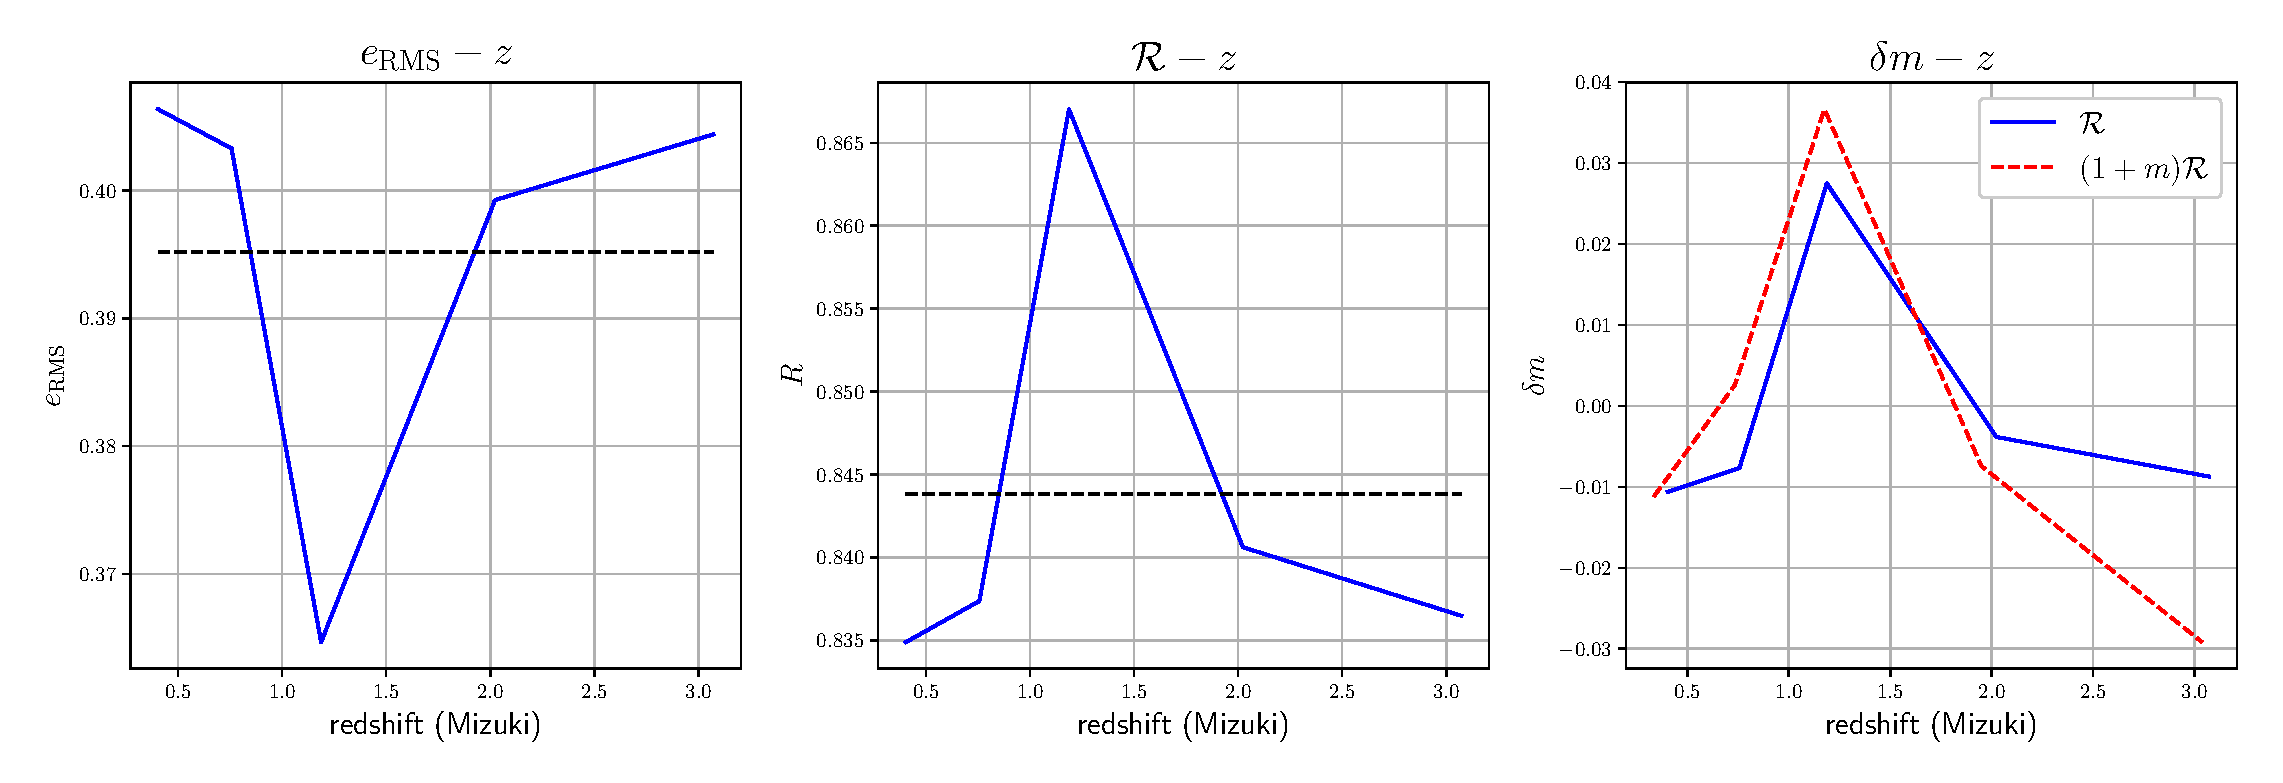
\includegraphics[width=0.9\textwidth]{redshift_dep_s16_vs_s19.eps}
% }
% \caption{The solid line in the left panel shows the redshift dependence of
%     intrinsic shape and the dashed line in the left panel shows the average
%     intrinsic shape. The solid line in the middle panel shows the redshift
%     dependence of responsivity and the dashed line in the middle panel shows
%     the average responsivity. The solid line shows in the right panel shows the
%     multiplicative bias residual due to the redshift dependence of responsivity
%     and the dashed line in the right panel shows the total multiplicative bias
%     residual.
%     }
% \end{figure*}
